\documentclass[letterpaper,12pt]{article}
\usepackage{tabularx} % extra features for tabular environment
\usepackage{amsmath}  % improve math presentation
\usepackage{float}
\usepackage{pdfpages}
\usepackage{cite}
\usepackage{multicol}
\usepackage{graphicx} % takes care of graphic including machinery
\graphicspath{ {./figures/} }
%\usepackage[margin=1in,letterpaper]{geometry} % decreases margins

\usepackage[final]{hyperref} % adds hyperlinks inside the generated pdf file
\hypersetup{
    colorlinks=true,       % false: boxed links; true: colored links
    linkcolor=blue,        % color of internal links
    citecolor=blue,        % color of links to bibliography
    filecolor=magenta,     % color of file links
    urlcolor =blue         
}
\usepackage[margin = 1in,headsep=0.5cm,headheight=2cm,letterpaper]{geometry} 
\usepackage{subcaption}

\usepackage{fancyhdr}

\usepackage{listings}
\usepackage{color}

\definecolor{dkgreen}{rgb}{0,0.6,0}
\definecolor{gray}{rgb}{0.5,0.5,0.5}
\definecolor{mauve}{rgb}{0.58,0,0.82}

\lstset{frame=tb,
  language=Python,
  aboveskip=3mm,
  belowskip=3mm,
  showstringspaces=false,
  columns=flexible,
  basicstyle={\small\ttfamily},
  numbers=none,
  numberstyle=\tiny\color{gray},
  keywordstyle=\color{blue},
  commentstyle=\color{dkgreen},
  stringstyle=\color{mauve},
  breaklines=true,
  breakatwhitespace=true,
  tabsize=3
}




\pagestyle{fancy}
\lhead{Intern: Ahmet Akman 2442366  \\ Supervisor: Dr. Johannes Zierenberg}
%\rhead{Date: \today \\ Duration: 19.07.22-21.08.22} 
%\cfoot{center of the footer!}
\renewcommand{\headrulewidth}{0.1pt}

\title{

\includegraphics[width=17cm]{odtu.png} \\

\includegraphics[width=4cm]{eee.png} \\
\vspace*{0.5in}
\textbf{EE400 Summer Practice Report}
\vspace*{0.25in}
}

\author{Intern: Ahmet Akman 2442366\\
Supervisor: Dr. Johannes Zierenberg\\
Supervisor Contact: \href{mailto: johannes.zierenberg@ds.mpg.de}{ johannes.zierenberg@ds.mpg.de. }-\href{tel:+495515176475}{+495515176475}\\
Assigned Faculty Member: Prof.Dr. Engin Tuncer\\
Institution Name: Max Planck Institute for Dynamics and Self-Organization\\
Start date:03.07.2023 || End date: 22.09.2023\\
        \vspace*{0.25in} \\
        Electrical and Electronics Engineering Department\\
        \textbf{Middle East Technical University}\\
        Ankara, Turkey
       } \date{\today}


\begin{document}

\bibliographystyle{plain}

%\thispagestyle{empty}
%\includepdf[pages=-]{coverpage_signed.pdf}


\maketitle

\newpage
\tableofcontents
\newpage
%\begin{abstract}
%abstract
%\end{abstract}
\section{Introduction}
\section{About Institution}
\subsection{Institution Name}
Max Planck Institute for Dynamics and Self-Organization.
\subsection{Institution Location}
Max Planck Institute for Dynamics and Self-Organization
Am Faßberg 17
37077 Göttingen
Germany
\subsection{General Description}
The Max Planck Institute for Dynamics and Self-Organization, located in Göttingen, Germany, is a prominent research institution primarily focused on the investigation of complex non-equilibrium systems, particularly within the fields of physics and biology. Its historical roots trace back to 1911 when Ludwig Prandtl initiated the establishment of a Kaiser Wilhelm Institute dedicated to the study of aerodynamics and hydrodynamics. This initial effort led to the formation of the Aeronautische Versuchsanstalt in 1915, which later evolved into the Kaiser Wilhelm Institute for Flow Research in 1924. In 1948, it became a part of the Max Planck Society. In 2003, it underwent a name change and became the Max Planck Institute for Dynamics and Self-Organization. Presently, it stands as one of the 80 institutes under the auspices of the Max Planck Society, contributing significantly to the understanding of intricate dynamic systems.

\subsection{Organization Structure}

\section{Project Background and Motivation}
The research project for the internship is constructed upon the following set of previous research. In the field of neuroscience \cite{CHAOS}, initiated the idea of inhibition is a necessary part of a neuronal network for stability of the network. Then, the impactful paper \cite{brunel} explained the dynamics of a sparsely connected random network with fixed parameters. Also, the role of inhibition was similar to the \cite{CHAOS}. The phases of the network through these dynamics are also stated. These states can be summarized as follows also givein in Figure \ref{brunel_fig}. Synchronous regular (SR) is the state where the whole network is blinking in a synchronized way. So, the neurons are synchronized with each other, exciting each other together, and regular activity is observed. Synchronous irregular (SI) is the state where the individual neurons show irregular activity, but the global activity is still regular. Therefore, the rate of the random network is still blinking in some sense. SI-fast and SI-slow characterize this as two different dynamical states. The asynchronous irregular state is the desired stable state where both the individual (per-neuron) and global activity show irregularity, that is, to small average overall activity not-blinking global network. \cite{brunel} has been considered as a guiding baseline in the field, and many other network descriptions built upon this idea, including inhibition as a factor for stability. It is important to note that the \cite{brunel} employs a fixed set of parameters on a completely randomly connected network.

\begin{figure}[htbp]
    \centering
    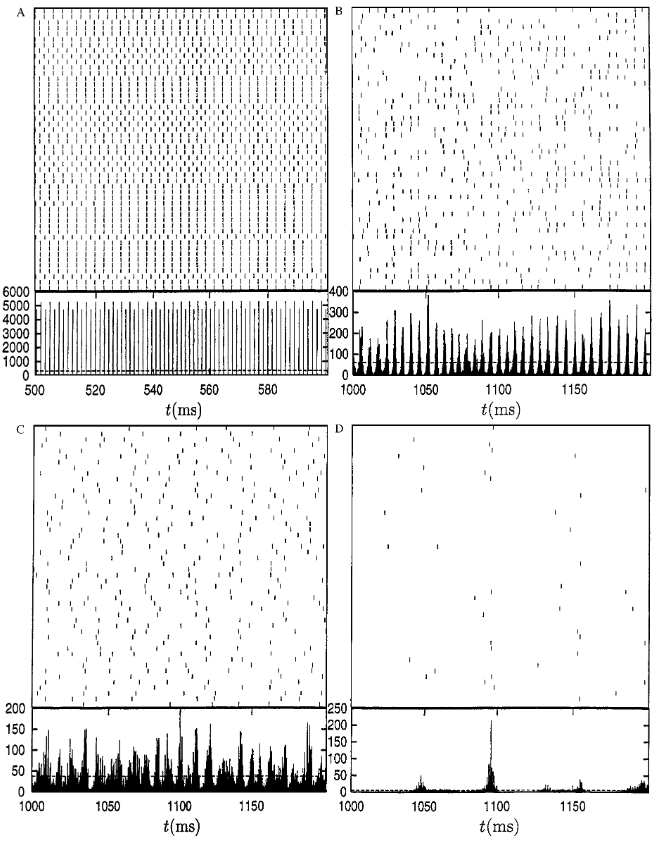
\includegraphics[width = 0.5\textwidth]{brunel.png}
    \caption{The states of the networks. (A) Synchronous Irregular. (B) Synchronous Irregular-fast. (C) Asynchronous Irregular. (D) Synchronous Irregular-slow.}
    \label{brunel_fig}
\end{figure} 

\subsection{Hypothesis}

In neurobiology, one can characterize the neurons as excitatory and inhibitory. A typical excitatory neuron is called a pyramidal neuron, whereas there are more than 20 mainstream types of inhibitory neurons. The idea is that the role of inhibition might be something other than only stabilizing the network. So, we hypothesize that only excitatory networks can be stable. To achieve this goal, the structural connectivity of the network should be reconsidered. \cite{2Dstructure} describes the 2D layered structure of the cortical networks in the brain. 
\section{Project Description}
\subsection{Baseline}
\subsection{Homeostastatic Regulation}
\subsection{Future Projection on the Project}

\section{Project Implementation and Results}
\subsection{Baseline Results}
\subsection{Homeostatic Regulation Results}

\section{Conclusion}
\section{References}
\bibliography{refs/cite}

\section{Appendix}

\end{document}

%%%%%%%%%%%%%%%%%%%%%%   EXAMPLE TABLE   %%%%%%%%%%%%%%%%%%%%%%%%%%%%%%%%
\begin{table}[H]
\begin{center}
    \caption{Resistance reading by color code convention.}
    \vspace{2mm}
    \begin{tabular}{||c | c | c||} 
        \hline
        Color Order & Value & Tolerance \\ [0.5ex] 
        \hline\hline
        Brown / Black / Red / Gold & 1k\( \Omega \) & \( \% \) 5  \\ 
        \hline
        Yellow / Violet / Red / Gold & 4.7k\( \Omega \) & \( \% \) 5   \\
        \hline
        Brown / Grey / Orange / Gold & 18k\( \Omega \) & \( \% \) 5  \\ [1ex] 
        \hline
    \end{tabular}
\end{center}
\end{table}


%%%%%%%%%%%%%%%%%%%%%%   EXAMPLE IMAGE   %%%%%%%%%%%%%%%%%%%%%%%%%%%%%%%%
\begin{figure}[H]
\centering
\includegraphics[width = 1\textwidth]{5.png}
\caption{Circuit schematic for step 5}
\end{figure} 

%%%%%%%%%%%%%%%%%%%%%%   EXAMPLE IMAGE FROM PDF   %%%%%%%%%%%%%%%%%%%%%%%%%%%%%%%%
\begin{figure}[H] \centering{
    \includegraphics[scale=0.25]{2a_plot.pdf}}
    \caption{Experiment 2}
\end{figure}
